\chapter{Realizace finálního prototypu}

%%TODO  Tato kapitola popisuje realizaci finálního prototypu měřiče impedance. Obecné principy použité v návrhu byly popsány v předchozích kapitolách, proto je zde pozornost věnována zejména konkrétnímu zapojení, zvoleným součástkám a změnám oproti prvnímu prototypu.

\section{Změny oproti testovacímu prototypu}

Hlavní změnou oproti testovacímu prototypu byl přechod z analogového vyhodnocování amplitudy a fáze na metodu přímého vzorkování měřených 
signálů popsanou v kapitole \ref{sec:digit_sampling}. 
Tím bylo možné odstranit část analogových vyhodnocovacích obvodů a přesunout výpočet impedance do mikrokontroléru.

Z tohoto důvodu byl změněn také řídicí mikrokontrolér. Místo ESP32-S2 byl použit STM32F103C8, 
který obsahuje dva 12bitové \acs{ADC} převodníky s dostatečnou vzorkovací rychlostí a podporou \acs{DMA} pro rychlé ukládání do paměti. 
Důležitou roli při výběru mikrokontroléru hrála také předchozí zkušenost s jeho použitím a dostupná podpora v prostředí Arduino.

V měřicí části byly použity rychlejší operační zesilovače OPA2192 \cite{OPA2192}, které by neměly zkreslovat signál při vyšších kmitočtech.

\section{Blokové zapojení zařízení}

Zařízení se skládá ze zdroje měřicího signálu, analogové měřicí části, mikrokontroléru a komunikačního rozhraní pro připojení k počítači. 
Měřicí signál je přiveden na měřenou součástku a proud procházející součástkou je převeden
 na napětí pomocí samovyvažovacího můstku a vybraného bočníku. 
 Napěťový i proudový kanál jsou dále zesíleny a jejich signály jsou vzorkovány pomocí \acs{A/D} převodníků mikrokontroléru.

\begin{figure}[H]
    \centering
    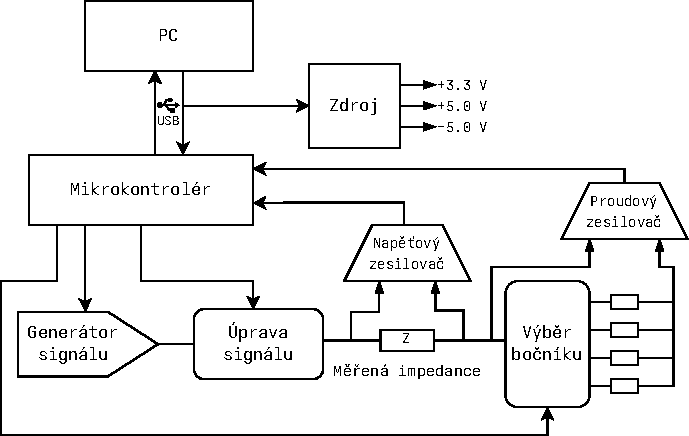
\includegraphics[width=0.95\textwidth]{obrazky/block_diagram_meter.pdf}
    \caption{Blokové schéma finálního prototypu měřiče impedance}
    \label{fig:finalni_blokove_schema}
\end{figure}

%% TODO:\section{Zdroj měřicího signálu}
%% 
%% Zdroj měřicího signálu vychází z principu přímé digitální syntézy popsaného v kapitole \ref{sec:dds}. Pro finální prototyp bylo zachováno řešení ověřené na prvním prototypu, protože generátor měřicího signálu pracoval spolehlivě i při maximální požadované frekvenci 100~kHz.
%% 
%TODO: V této části je vhodné doplnit konkrétní hodnoty použitých součástek, rozsah nastavení amplitudy, způsob nastavení stejnosměrné složky a případné rozdíly proti prvnímu prototypu.


\section{Návrh desky plošných spojů}

Finální prototyp byl realizován na 6-vrstvé desce plošných spojů. 
Návrh desky musel zohlednit oddělení analogové a digitální části, 
krátké vedení citlivých měřicích signálů a vhodné umístění napájecích blokovacích kondenzátorů. 
Součástky byly seskupeny do jednotlivých funkčních bloků, viz obr.~\ref{fig:finalni_navrh_dps}.

Signální cesty byly zapojeny na vnějších měděných vrstvách z důvodu snadného přístupu pro budoucí opravy, zatímco 
vnitřní 4 vrstvy byly použity jako souvislé plochy pro nízkoimpedanční připojení napájení ke všem součástkám.
Většina pasivních součástek byla umístěna na zadní stranu desky.


\begin{figure}[H]
    \centering
    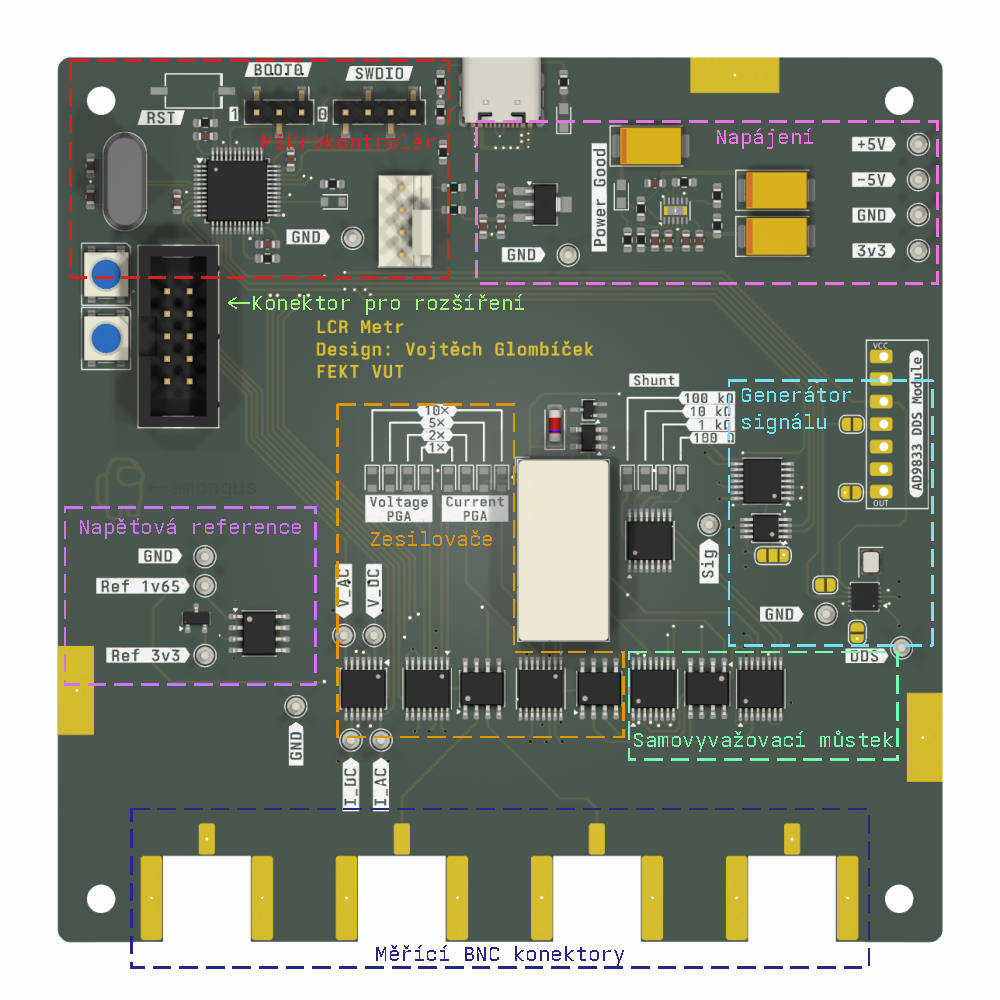
\includegraphics[width=0.95\textwidth]{obrazky/layout_img.pdf}
    \caption{Render navržené DPS s vyznačenými funkčními bloky.}
    \label{fig:finalni_navrh_dps}
\end{figure}




\subsection{Ruční opravy desky}

Při oživování byly zjištěny chyby návrhu desky, které byly v prototypu opraveny ručními úpravami (viz obr.~\ref{fig:finalni_pcb_foto}).

\begin{enumerate}
    \item Nesprávné zapojení neinvertujícího sumačního zesilovače bylo opraveno odstraněním rezistorů ze spodní strany desky a přidáním nových na horní stranu.
    \item Zaměněné vstupy \acs{OZ} byly opraveny nadzvednutím pinů čipu a správným připojením drátky. Původní plošky byly izolovány kaptonovou páskou.
    \item Původní návrh rozděloval výstup diferenčního zesilovače na dva, z nichž jeden byl filtrován dolní a druhý horní propustí. Nebylo však zohledněno, že \acs{HP} odstraní fixní DC složku potřebnou pro vstup do \acs{ADC}, který neměří záporné napětí. Tato chyba byla opravena přemostěním filtrů, nyní se měří přímo signál z diferenčního zesilovače. 
   % \item Označení indikačních LED pro zesílení napětí je zrcadlené, ale rozmístění jednotlivých LED zrcadlené není. Tato chyba nebyla opravena, nemá vliv na funkčnost.
\end{enumerate}

Všechny tyto chyby byly způsobeny nepozorností při návrhu schématu. Schéma uvedené v příloze bylo opraveno.

\begin{figure}[H]
    \centering
    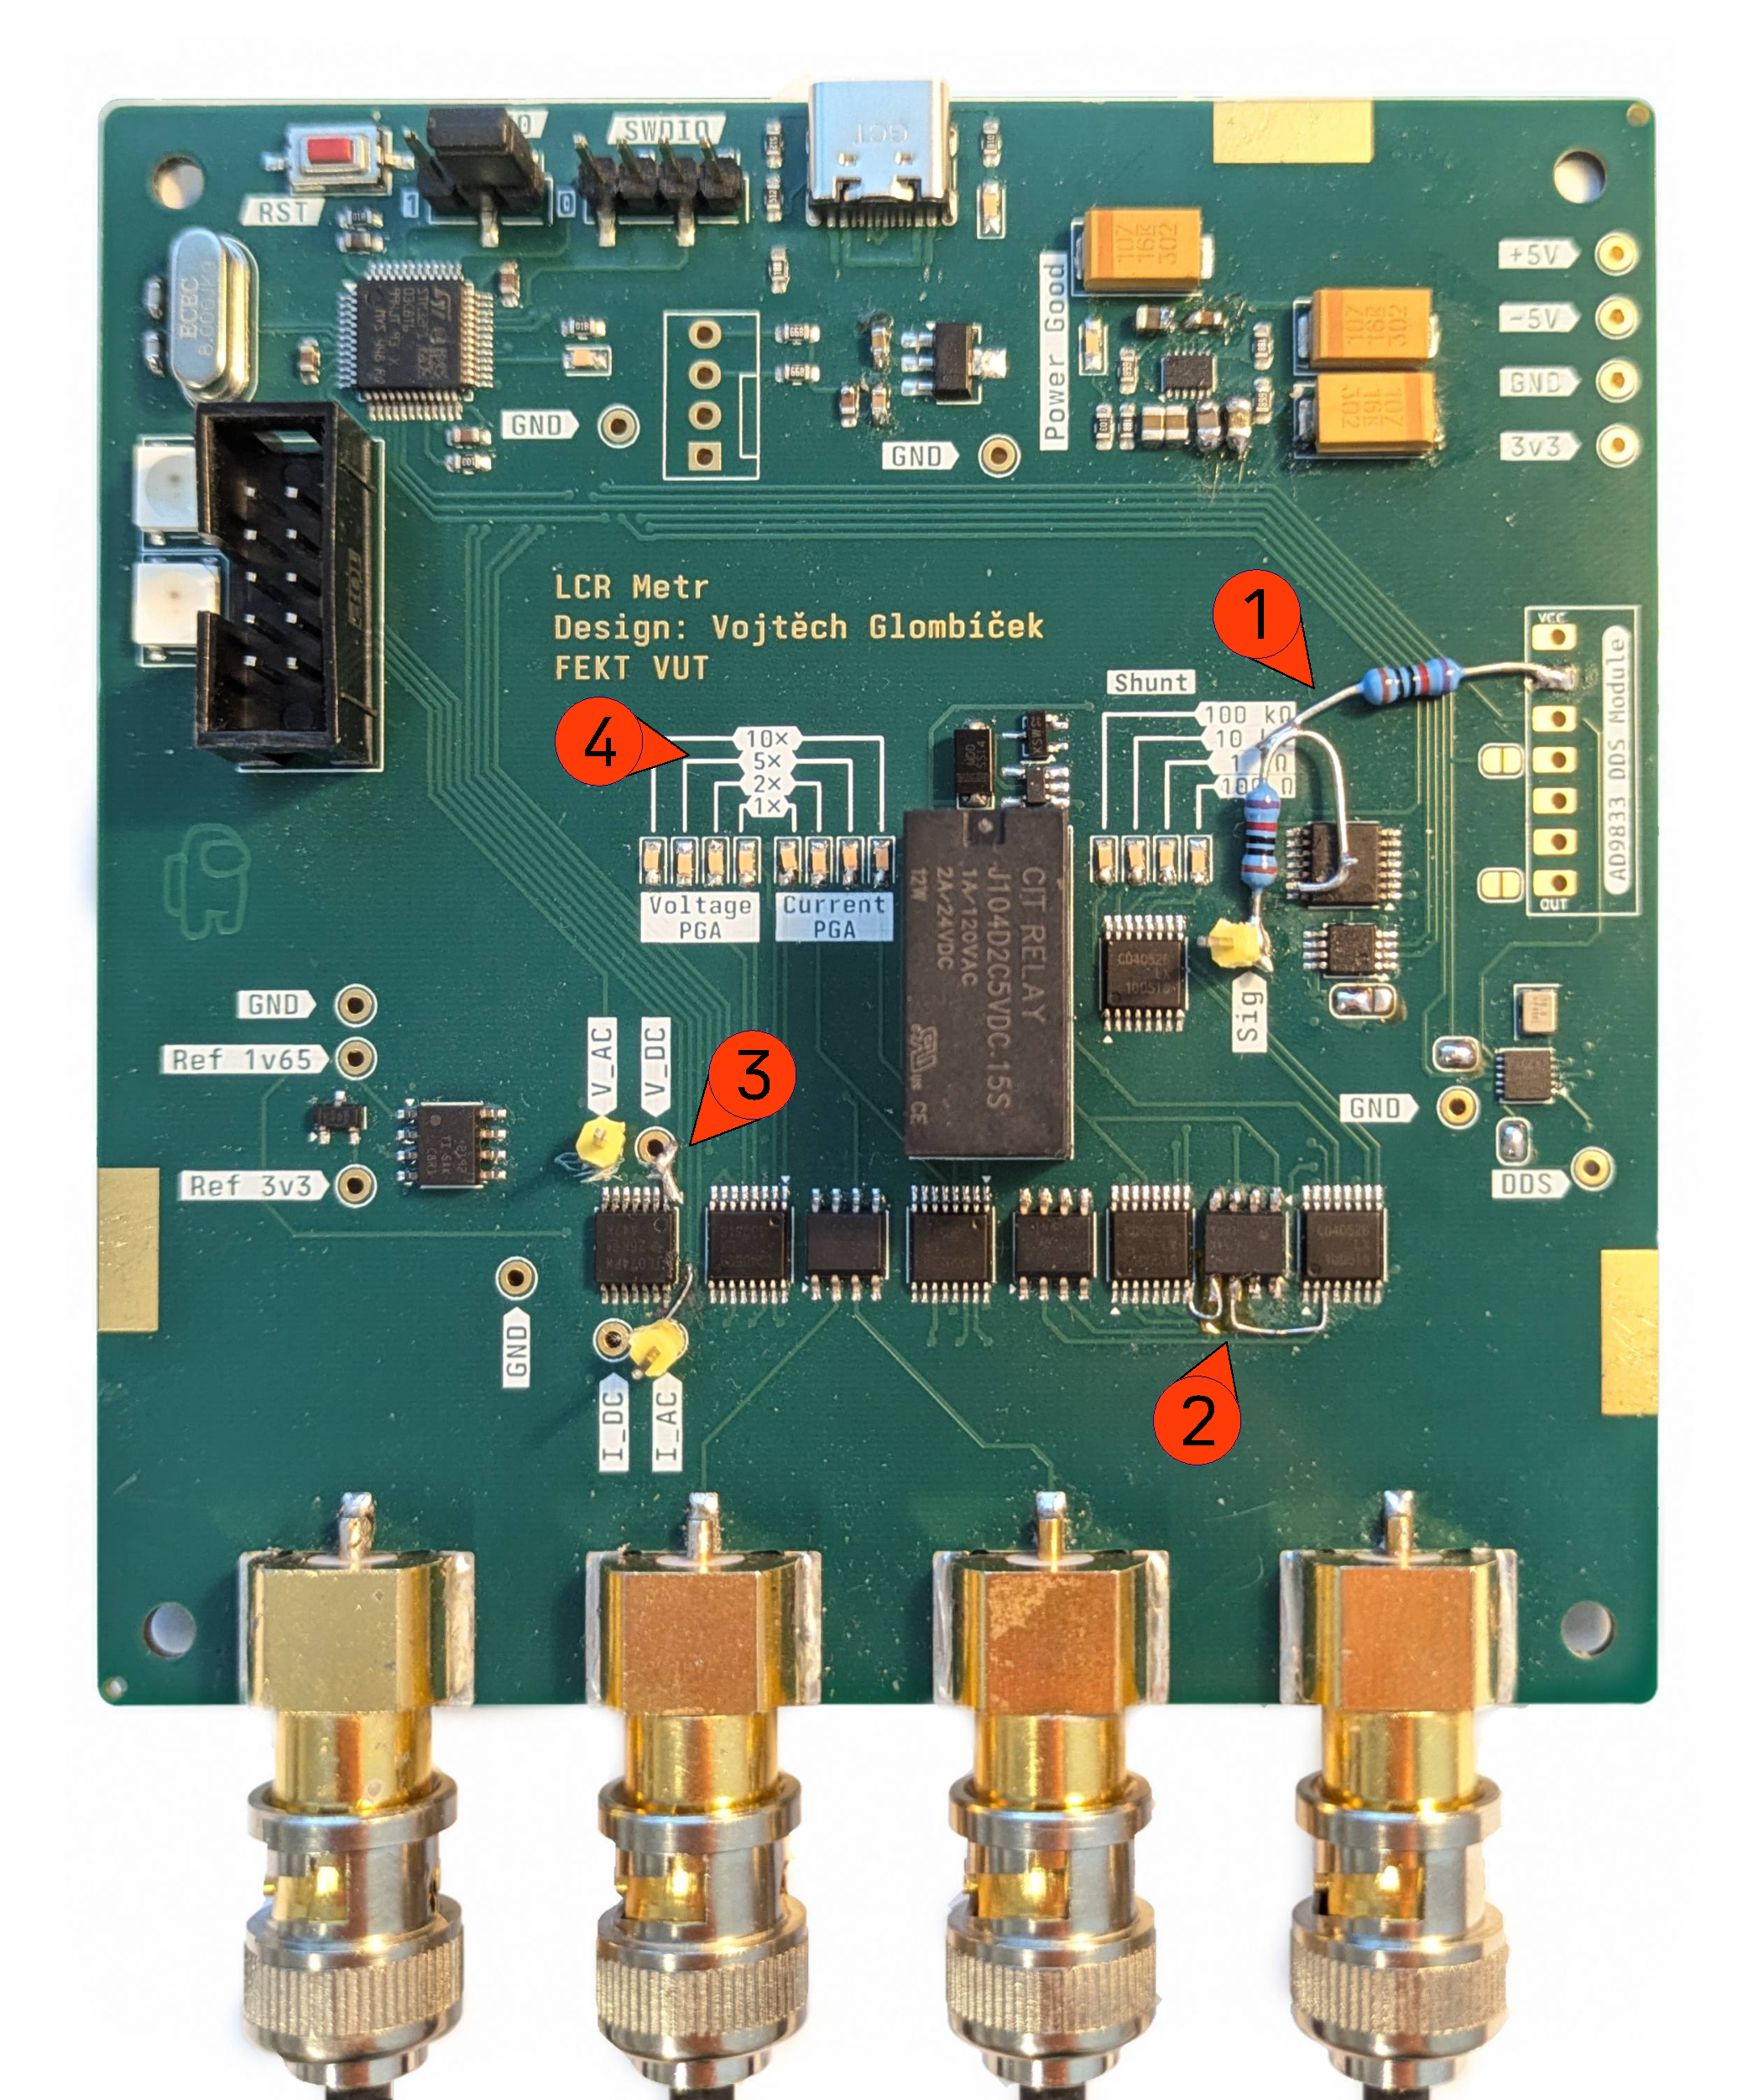
\includegraphics[width=0.9\textwidth]{obrazky/final_PCB_photo_marked.pdf}
    \caption{Osazená DPS finálního prototypu s označenými ručními opravami.}
    \label{fig:finalni_pcb_foto}
\end{figure}